\documentclass[12pt,a4paper]{article}
\usepackage{graphicx}
\usepackage{apacite}
\usepackage{amsmath}
\usepackage{relsize}
\usepackage{float}
\usepackage{inputenc}
\usepackage{csquotes}
\usepackage{amsmath}
\usepackage{mathdots}
\usepackage[toc,page]{appendix}
\usepackage{caption}
\usepackage{amssymb}
\usepackage{pdfpages}
\usepackage{subcaption}
\usepackage{gensymb}
\usepackage[margin=0.5in]{geometry}
\usepackage{subcaption}
\setlength\parindent{0pt}
\usepackage{wrapfig}
\usepackage{multicol}

\begin{document}
\begin{titlepage}
	\begin{center}
	\line(1,0){200}\\
	[0.25in]
	\huge{\bfseries COMP20003 \\Algorithms and Data Structures}\\
	[2mm]
	\line(1,0){200}\\
	[1.5cm]
	\textsc{\LARGE Assignment \#3 - Experimentation}\\
	[17.5cm]
	\end{center}

	\begin{flushright}	
	\textsc{ Goh Xing Yang\\}
	\# 1001969\\
	
	October 29, 2020\\
	\end{flushright}
\end{titlepage}

\pagenumbering{arabic}
\setcounter{page}{1}




\section{Experimentation Data}
\begin{table}[H]
\caption{Statistics for Layout 0 (3 Pegs)}
\label{tab:my-table}

\begin{tabular}{|c|c|c|c|c|c|}
\hline
Budget  & \multicolumn{1}{l|}{Pegs Left} & \multicolumn{1}{l|}{Generated Nodes} & \multicolumn{1}{l|}{Expanded Nodes} & \multicolumn{1}{l|}{Expanded/Sec} & \multicolumn{1}{l|}{Execution   Time (Sec)} \\ \hline
10000   & 1                              & 2                                    & 2                                   & 50                                   & 0.039493                                              \\ \hline
100000  & 1                              & 2                                    & 2                                   & 50                                   & 0.039493                                              \\ \hline
1000000 & 1                              & 2                                    & 2                                   & 50                                   & 0.039493                                              \\ \hline
1500000 & 1                              & 2                                    & 2                                   & 50                                   & 0.039493                                              \\ \hline
\end{tabular}
\end{table}

Layout 0 only requires 2 expanded nodes in the Depth First Search (DFS) to achieve a winning solution so a budget of 10000 is sufficient, therefore, increasing the budget has no effect on the solution.\\


\begin{table}[H]
\caption{Statistics for Layout 1 (4 Pegs)}
\label{tab:my-table}

\begin{tabular}{|c|c|c|c|c|c|}
\hline
Budget  & \multicolumn{1}{l|}{Pegs Left} & \multicolumn{1}{l|}{Generated Nodes} & \multicolumn{1}{l|}{Expanded Nodes} & \multicolumn{1}{l|}{Expanded/Sec} & \multicolumn{1}{l|}{Execution Time (Sec)} \\ \hline
10000   & 1                              & 3                                    & 3                                   & 71                                   & 0.042087                                              \\ \hline
100000  & 1                              & 3                                    & 3                                   & 71                                   & 0.042087                                              \\ \hline
1000000 & 1                              & 3                                    & 3                                   & 71                                   & 0.042087                                              \\ \hline
1500000 & 1                              & 3                                    & 3                                   & 71                                   & 0.042087                                              \\ \hline
\end{tabular}
\end{table}
Layout 1 only requires 3 expanded nodes in the DFS to achieve a winning solution so a budget of 10000 is sufficient, therefore, increasing the budget has no effect on the solution.\\

\begin{table}[H]
\caption{Statistics for Layout 2 (7 Pegs)}
\label{tab:my-table}

\begin{tabular}{|c|c|c|c|c|c|}
\hline
Budget  & \multicolumn{1}{l|}{Pegs Left} & \multicolumn{1}{l|}{Generated Nodes} & \multicolumn{1}{l|}{Expanded Nodes} & \multicolumn{1}{l|}{Expanded/Sec} & \multicolumn{1}{l|}{Execution Time (Sec)} \\ \hline
10000   & 1                              & 8                                    & 7                                   & 172                                  & 0.04055                                               \\ \hline
100000  & 1                              & 8                                    & 7                                   & 172                                  & 0.04055                                               \\ \hline
1000000 & 1                              & 8                                    & 7                                   & 172                                  & 0.04055                                               \\ \hline
1500000 & 1                              & 8                                    & 7                                   & 172                                  & 0.04055                                               \\ \hline
\end{tabular}
\end{table}
Layout 2 only requires 7 expanded nodes in the DFS to achieve a winning solution so a budget of 10000 is sufficient, therefore, increasing the budget has no effect on the solution.\\

\begin{table}[H]
\caption{Statistics for Layout 3 (17 Pegs)}
\label{tab:my-table}

\begin{tabular}{|c|c|c|c|c|c|}
\hline
Budget  & \multicolumn{1}{l|}{Pegs Left} & \multicolumn{1}{l|}{Generated Nodes} & \multicolumn{1}{l|}{Expanded Nodes} & \multicolumn{1}{l|}{Expanded/Sec} & \multicolumn{1}{l|}{Execution Time (Sec)} \\ \hline
10000   & 1                              & 10282                                & 3541                                & 77307                                & 0.045804                                              \\ \hline
100000  & 1                              & 10282                                & 3541                                & 77307                                & 0.045804                                              \\ \hline
1000000 & 1                              & 10282                                & 3541                                & 77307                                & 0.045804                                              \\ \hline
1500000 & 1                              & 10282                                & 3541                                & 77307                                & 0.045804                                              \\ \hline
\end{tabular}
\end{table}
Layout 3 only requires 3541 expanded nodes in the DFS to achieve a winning solution so a budget of 10000 is sufficient, therefore, increasing the budget has no effect on the solution.\\

\begin{table}[H]
\caption{Statistics for Layout 4 (32 Pegs)}
\label{tab:my-table}

\begin{tabular}{|c|c|c|c|c|c|}
\hline
Budget  & \multicolumn{1}{l|}{Pegs Left} & \multicolumn{1}{l|}{Generated Nodes} & \multicolumn{1}{l|}{Expanded Nodes} & \multicolumn{1}{l|}{Expanded/Sec} & \multicolumn{1}{l|}{Execution Time (Sec)} \\ \hline
10000   & 1                              & 2418                                 & 1065                                & 27005                                & 0.039436                                              \\ \hline
100000  & 1                              & 2418                                 & 1065                                & 27005                                & 0.039436                                              \\ \hline
1000000 & 1                              & 2418                                 & 1065                                & 27005                                & 0.039436                                              \\ \hline
1500000 & 1                              & 2418                                 & 1065                                & 27005                                & 0.039436                                              \\ \hline
\end{tabular}
\end{table}
Layout 4 only requires 1065 expanded nodes in the DFS to achieve a winning solution so a budget of 10000 is sufficient, therefore, increasing the budget has no effect on the solution.\\

\begin{table}[H]
\caption{Statistics for Layout 5 (36 Pegs)}
\label{tab:my-table}

\begin{tabular}{|c|c|c|c|c|c|}
\hline
Budget  & \multicolumn{1}{l|}{Pegs Left} & \multicolumn{1}{l|}{Generated Nodes} & \multicolumn{1}{l|}{Expanded Nodes} & \multicolumn{1}{l|}{Expanded/Sec} & \multicolumn{1}{l|}{Execution Time (Sec)} \\ \hline
10000   & 4                              & 26495                                & 10000                               & 167112                               & 0.05984                                               \\ \hline
100000  & 3                              & 359818                               & 100000                              & 325157                               & 0.307543                                              \\ \hline
1000000 & 2                              & 4488464                              & 1000000                             & 302302                               & 3.307949                                              \\ \hline
1500000 & 1                              & 4898609                              & 1090275                             & 305827                               & 3.565004                                              \\ \hline
\end{tabular}
\end{table}
Winning solution found using 1.5M budget, with 1090275 expanded nodes required. Effects of the budget on the number of pegs left is plotted below:
\begin{figure}[H]
\centering
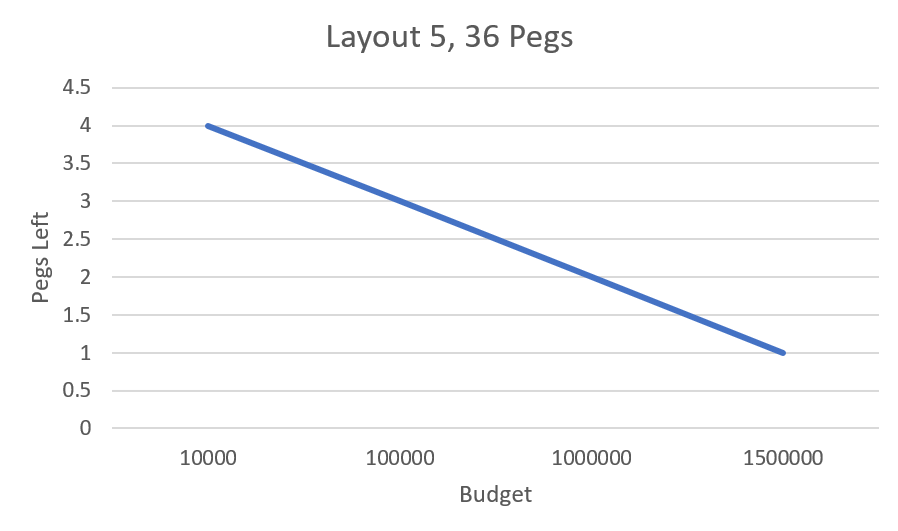
\includegraphics[scale=0.5]{layout5.png}
\caption{Budget vs number of pegs left for layout 5}
\end{figure}

\begin{table}[H]
\caption{Statistics for Layout 6 (44 Pegs)}
\label{tab:my-table}

\begin{tabular}{|c|c|c|c|c|c|}
\hline
Budget  & \multicolumn{1}{l|}{Pegs Left} & \multicolumn{1}{l|}{Generated Nodes} & \multicolumn{1}{l|}{Expanded Nodes} & \multicolumn{1}{l|}{Expanded/Sec} & \multicolumn{1}{l|}{Execution Time (Sec)} \\ \hline
10000   & 5                              & 29368                                & 10000                               & 149485                               & 0.066896                                              \\ \hline
100000  & 4                              & 374378                               & 100000                              & 324315                               & 0.308342                                              \\ \hline
1000000 & 3                              & 4481233                              & 1000000                             & 316826                               & 3.156305                                              \\ \hline
1500000 & 3                              & 7020668                              & 1500000                             & 298157                               & 5.030905                                              \\ \hline
\end{tabular}
\end{table}

Unable to find winning solution within 1.5M budget. Effects of the budget on the number of pegs left plotted is below:

\begin{figure}[H]
\centering
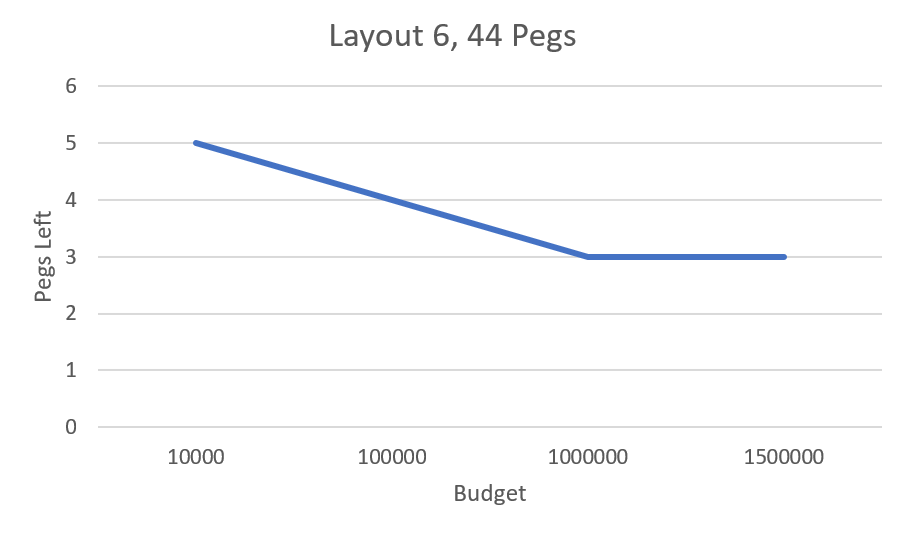
\includegraphics[scale=0.5]{layout6.png}
\caption{Budget vs number of pegs left for layout 6}
\end{figure}



\begin{table}[H]
\caption{Statistics for Layout 7 (38 Pegs)}
\label{tab:my-table}

\begin{tabular}{|c|c|c|c|c|c|}
\hline
Budget  & \multicolumn{1}{l|}{Pegs Left} & \multicolumn{1}{l|}{Generated Nodes} & \multicolumn{1}{l|}{Expanded Nodes} & \multicolumn{1}{l|}{Expanded/Sec} & \multicolumn{1}{l|}{Execution Time (Sec)} \\ \hline
10000   & 4                              & 32469                                & 10000                               & 156071                               & 0.064073                                              \\ \hline
100000  & 2                              & 386440                               & 100000                              & 314414                               & 0.318051                                              \\ \hline
1000000 & 2                              & 4790308                              & 1000000                             & 297929                               & 3.356498                                              \\ \hline
1500000 & 2                              & 7173504                              & 1500000                             & 278817                               & 5.37987                                               \\ \hline
\end{tabular}
\end{table}
Unable to find winning solution within 1.5M budget. Effects of the budget on the number of pegs left plotted is below:

\begin{figure}[H]
\centering
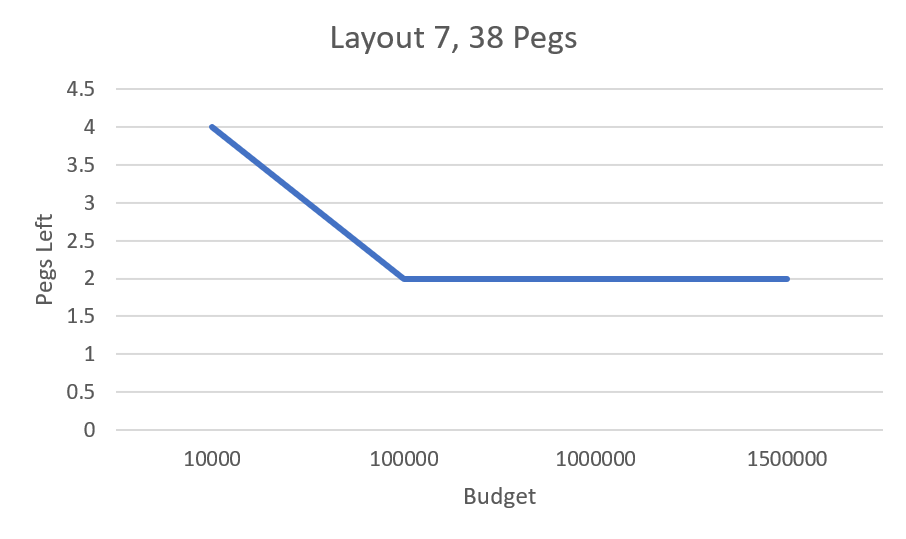
\includegraphics[scale=0.5]{layout7.png}
\caption{Budget vs number of pegs left for layout 7}
\end{figure}

\begin{table}[H]
\caption{Statistics for Layout 8 (40 Pegs)}
\label{tab:my-table}

\begin{tabular}{|c|c|c|c|c|c|}
\hline
Budget  & \multicolumn{1}{l|}{Pegs Left} & \multicolumn{1}{l|}{Generated Nodes} & \multicolumn{1}{l|}{Expanded Nodes} & \multicolumn{1}{l|}{Expanded/Sec} & \multicolumn{1}{l|}{Execution Time (Sec)} \\ \hline
10000   & 6                              & 27562                                & 10000                               & 167383                               & 0.059743                                              \\ \hline
100000  & 4                              & 349921                               & 100000                              & 320955                               & 0.31157                                               \\ \hline
1000000 & 4                              & 4073028                              & 1000000                             & 328191                               & 3.046998                                              \\ \hline
1500000 & 4                              & 6361454                              & 1500000                             & 299354                               & 5.010775                                              \\ \hline
\end{tabular}
\end{table}
Unable to find winning solution within 1.5M budget. Effects of the budget on the number of pegs left plotted is below:

\begin{figure}[H]
\centering
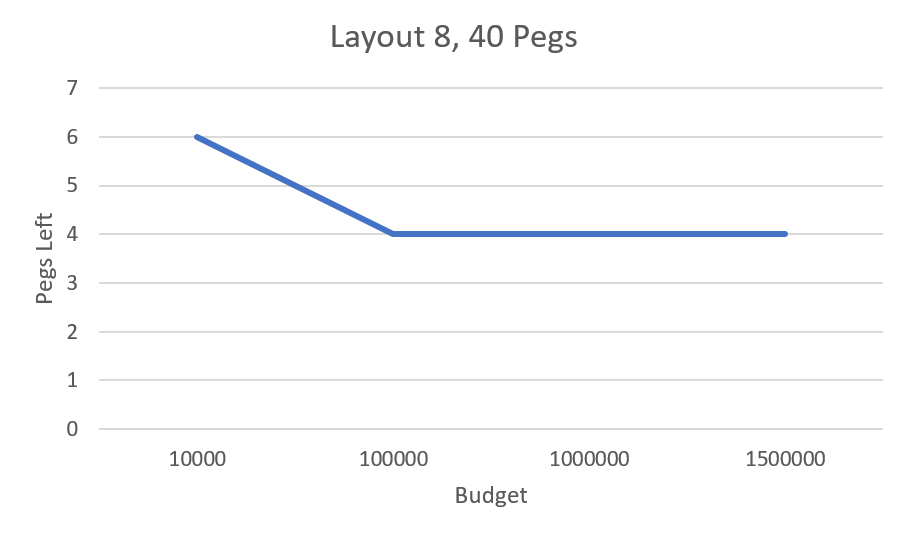
\includegraphics[scale=0.5]{layout8.png}
\caption{Budget vs number of pegs left for layout 8}
\end{figure}
Compiling the data into figures and plotting the effects of the budget on the solution for various layouts:

\begin{figure}[H]
\centering
\begin{subfigure}{.5\textwidth}
  \centering
  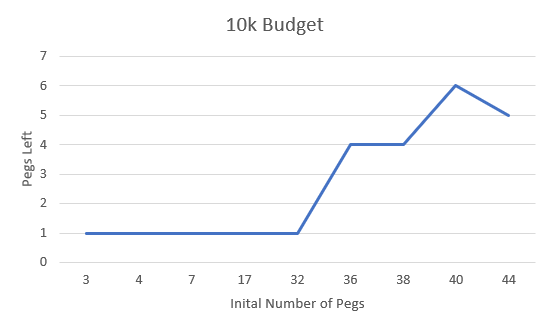
\includegraphics[width=1\linewidth]{10k.png}
  \caption{Budget = 10k}
  \label{fig:sub1}
\end{subfigure}%
\begin{subfigure}{.5\textwidth}
  \centering
  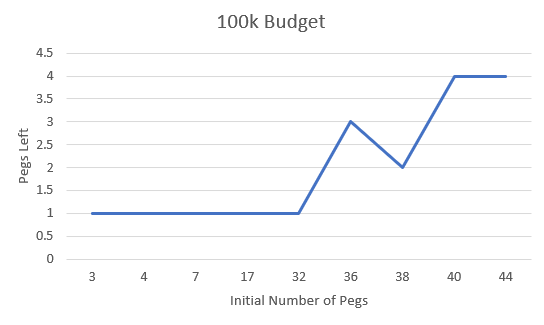
\includegraphics[width=1\linewidth]{100k.png}
  \caption{Budget = 100k}
  \label{fig:sub2}
\end{subfigure}
\begin{subfigure}{.5\textwidth}
  \centering
  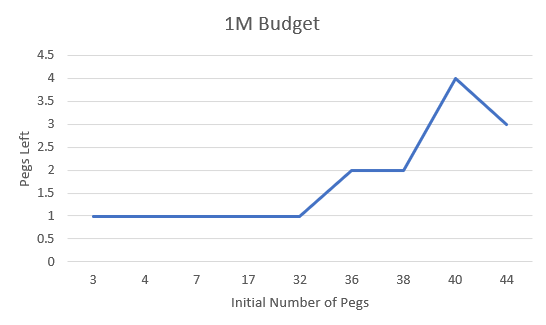
\includegraphics[width=1\linewidth]{1M.png}
  \caption{Budget = 1M}
  \label{fig:sub1}
\end{subfigure}%
\begin{subfigure}{.5\textwidth}
  \centering
  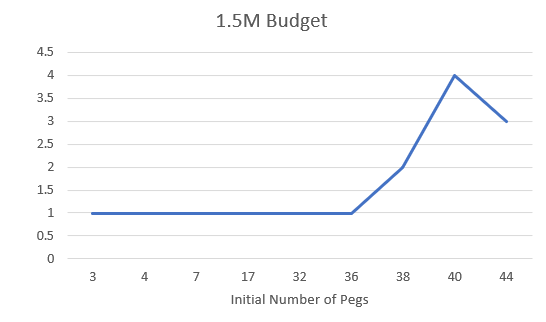
\includegraphics[width=1\linewidth]{1.5M.png}
  \caption{Budget = 1.5M }
  \label{fig:sub2}
\end{subfigure}
\caption{Initial number of pegs vs pegs left for various budgets}
\label{fig:test}
\end{figure}
As the budget increases, the number of pegs left move towards 1, however, this convergence generally becomes much slower as the number of initial pegs increase. With a sufficient budget, all the board states (initial pegs) would converge towards one, however, with a high number of initial pegs this computation can quickly become infeasible in terms of time using current computing methods.

\section{Discussion}
For the first 5 layouts, a budget of 10000 is sufficient to converge to a winning solution, therefore, an increased budget does not change the number of generated nodes. An important note is that the DFS strategy is a brute force method that cycles between the left-right-up-down moves starting from (0,0) to (9,9). This search does not use any heuristics to guide the search towards the solution and will always generate and expand the same number of nodes when executed with the same input.
\\

This DFS strategy means that the initial number of pegs is not the sole factor in determining the runtime, with the initial board layout position and number of permutations playing a large factor in the number of nodes expanded/generated. An example of this is between layout 3 and layout 4, with 17 and 32 pegs respectively. Although layout 3 has almost half the number of pegs as layout 4, it converges to the winning solution with only 1065 node expansions when compared to the 3541 node expansions required for layout 3, a factor of $\approx3.32$. This effect is also seen when comparing the best solution of layout 6 and layout 8 using a budget of 1.5M, where layout 6 contains 44 pegs initially and converges to 3 remaining pegs, however, layout 8 which contains 40 pegs only converges to 4 remaining pegs.
\\

For optimisations, a board position that can be flipped or rotated into another board position are considered identical, so checking this condition which runs in $\theta(n^2)$ time before inserting unique board states into the hash-table and stack will reduce the number of node expansions required.
\\



\end{document}
